\ei

 \subsection{Task 1: Study and understand the robustness factors of deep neural networks.}\label{4.1}


Previous efforts have focused on the data impacts of DNN robustness, however, fewer studies towards a holistic understanding of a wider range of configurations (e.g., model parameters and structure) and their coalesced effects with imperfect data for DNN robustness. 
In this task, we aim to systematically analyze the influence of each factor and their combinations (composition effects) on the robustness of DNN model in a range of downstream domains including image classification, video motion recognition, and medical diagnosis in Table~\ref{tab:existing}. 

In Table~\ref{tab:factors}, we consider the perturbation surface (i.e., data ($F_D$) and configuration ($F_C$)) and their specific modification targets, i.e., input, output, model parameter and structure. 
For each factor $F_i \in $ \{ $F_1$, $\dots$, $F_N$ \}, 
it has a set $T_{F_i}$ of modifications, including changing inputs, outputs and configurations to different pre-defined values. 
We use $\omega \subseteq T_{F_1}\dots\times T_{F_i}\dots \times T_{F_N}$ to represent a \emph{perturbation strategy}, which is a subset of all modifications given all factors combined. Hence we can train and produce different DNN models (e.g., $\mathcal{M}$) based on individual strategies (e.g., $\omega$) 

\begin{equation}
\label{eq:perturb_train}
    \mathcal{M}=train(\hat{\mathbb{X}},\hat{\mathbb{Y}}, \hat{\Theta}), \quad  s.t. \ \
    \hat{\mathbb{X}},\hat{\mathbb{Y}}, \hat{\Theta} = perturb_{\omega}(\mathbb{X},\mathbb{Y},\Theta),
\end{equation}
where $\hat{\mathbb{X}}, \hat{\mathbb{Y}}, \hat{\Theta}$ are modified inputs, outputs and configurations based on the strategy $\omega$.

\begin{wraptable}{r}{9.7cm}
\vspace{-5mm}
     \caption{\footnotesize Robustness affecting factors}
     \footnotesize
    \begin{tabular}{llc}
    \toprule
        \textbf{Surface} & \textbf{Factor} & \textbf{Modification Target}\\\midrule
        \multirow{3}{*}[-0.5\dimexpr \aboverulesep + \belowrulesep + \cmidrulewidth]{Data ($F_D$)} & $F_1$ Adversarial attack &  Input $\mathbb{X}$ \\\cline{2-3}
                        &$F_2$ Label flipping attack & \multirow{2}{*}[-0.5\dimexpr \aboverulesep + \belowrulesep + \cmidrulewidth]{Output $\mathbb{Y}$} \\ 
                        &$F_3$ Label noise injection  \\ \midrule
        \multirow{4}{*}[-0.5\dimexpr \aboverulesep + \belowrulesep + \cmidrulewidth]{ Configuration ($F_C$)}& $F_4$ Weight perturbation   & \multirow{4}{*}{Model $\Theta$ } \\ 
                       & $F_5$ Bias perturbation  &        \\
                       & $F_6$ Conv layer modification\tnote{1}&  \\
                       & $F_7$ FC layer modification\tnote{2} & \\
                        $\ldots$ &$\ldots$ &$\ldots$ \\
   \bottomrule
    \end{tabular}
    \label{tab:factors}
\end{wraptable}

Given $N$ factors with each having $T$ modifications, we will have combinations of $2^{T*N}$ perturbation strategies to exercise and test the robustness of a DNN model during its training. This search space is huge when trying to determine which strategy is more effective to degrade the robustness of the model, while the exhaustive enumeration in this search space by using the traditional methods (e.g. grid search) is time-consuming and labor-intensive. 
To alleviate the combinatorial explosion problem, we will investigate a differential evolution (\textbf{DE}) approach to capture cumulative confidence decision boundary (\textbf{C-CDD}) by selectively and iteratively searching the top-$Q$ most influential perturbation strategies.

\begin{wrapfigure}{l}{9.5cm}
    \centering
        \vspace{-3mm}
    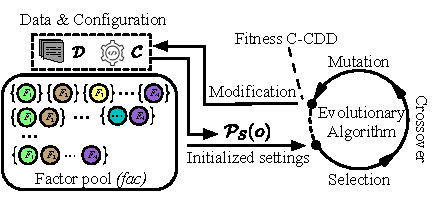
\includegraphics[scale=1]{fig/Task1.pdf}
    \vspace{-3mm}
    \caption{\footnotesize Differential Evolution Configuration}
    \label{fig:task1frame}
\end{wrapfigure}


\textbf{C-CDD.} Deep learning aims to predict the class of a sample $x\in\mathbb{X}$ by estimating the probability $p_{\mathcal{M}}(y\ |\ x)$ on each class by a model $\mathcal{M}$ which is trained based on Equation~\ref{eq:perturb_train}. \emph{Cumulative confidence decision boundary} (C-CDD) as defined in Equation~\ref{eq:cumlativeCDD} is used to estimate $\mathcal{M}$'s robustness by measuring the confidence of all predicted samples in $\mathbb{X}$. 
C-CDD reflects the relative distance of the inputs from the decision boundary to the human desired classes. 
A lower C-CDD score indicates that the model potentially has higher uncertainties (less robust) in its predictions. 
%To further shrink the search space, smaller modifications from fewer factors are always preferable if it has a similar C-CDD score as that of more modifications. 

\begin{equation}\label{eq:cumlativeCDD}
  \text{C-CDD} (\mathbb{X}, \mathcal{M})=  \mathbb{E}_{x\in\mathbb{X}}(p_{\mathcal{M}}(i\ |\ x)-p_{\mathcal{M}}(j\ |\ x)),
\end{equation}
where $\mathbb{E}$ denotes the expectation operation, $i$ denotes the human desired class and $j$ is the predicted class with the maximum prediction probability. 


\textbf{DE.} \emph{differential evolution} (DE)~\cite{DBLP:conf/ijcai/AwadMH21} is a fast global optimization algorithm to guide the search of the optimal perturbation strategies that perturb the DNN model effectively. 
Initially, we randomly generate a population of $Q$ strategies as the first generation. 
$\omega_i^g$ denotes $i$-th ($1 < i \leq Q$) strategy in the $g$-th generation. 
DE aims to optimize and mutate the $Q$ strategies in multiple generations in an evolutionary manner with a gradually reduced C-CDD score until a generation that produces the model has the lowest or a pre-defined C-CDD score. 


% \begin{figure}[!h]
%     \centering
%     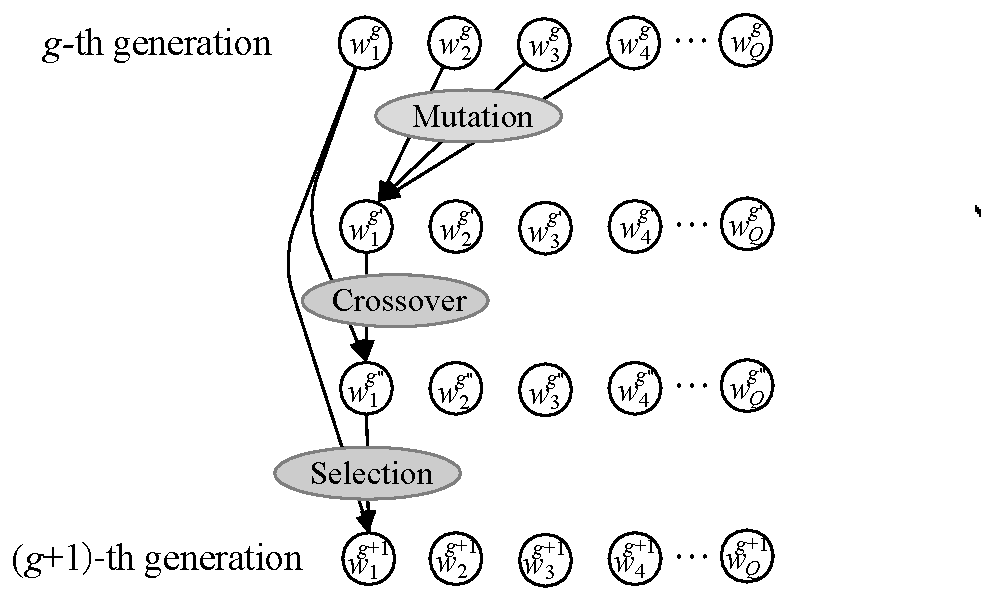
\includegraphics[width=9cm]{fig/DE.pdf}
%     \caption{population generation in DE.}
%     \label{fig:goal2}
% \end{figure}

For $\forall \omega_i^{g+1}$ in $(g+1)$-th generation, DE conducts the following four steps in order: 
\begin{enumerate}
    \item Generate. Three strategies $\omega_{r_1}^g$, $\omega_{r_2}^g$, $\omega_{r_3}^g$ are randomly selected from the population in $g$-th generation. The generated indexes must be distinct from each other and also different from the strategy index $i$ in $(g+1)$-th generation, i.e., $r_1 \neq r_2 \neq r_3 \neq i$.
    \item Mutate. The strategy for the $(g+1)$-th generation in the population is mutated by $\omega_i^{g+1} = \omega_{r_1}^g + \epsilon (\omega_{r_2}^g-\omega_{r_3}^g)$, where $\omega_{r_1}^g$, $\omega_{r_2}^g$, $\omega_{r_3}^g$ are generated from Step 1, and $\epsilon\in(0,1]$ denotes a scaling coefficient.
    \item Crossover. The strategy can be treated as a $K$-length vector that contains a sequence of  modification methods. Let $\omega_i^g[j]$ denote the $j$-th ($1\leq j \leq K$) modification in the perturbation strategy. 
    The crossover follows a random probability value from the uniform distribution, i.e., $r_i^{g}[j] \sim U(0,1)$. The $(g+1)$-th generation of each particular modification in the perturbation strategy can be obtained as: 
    \begin{equation}
    \omega_i^{g+1}[j] = \left\{ 
     \begin{array}{ll}
           \omega_i^{g}[j], & if\ r_i^{g+1}[j] < p_r \\ 
           \omega_i^{g+1}[j],& otherwise
     \end{array}
     \right. 
    \end{equation}
    Here, $p_r$ is a user-specified replacement rate (e.g.,  $0.9$).
    
    \item Select. For each newly generated strategy $\omega_i^{g+1}$, we produce a different DNN model by Equation~\eqref{eq:perturb_train} and select between $\omega_i^{g}$ and $\omega_i^{g+1}$ based on a lower C-CDD score calculated by Equation~\eqref{eq:cumlativeCDD}. 

\end{enumerate}

Given the top-$Q$ strategies and their trained models produced by DE, we will exploit effective methods of robustness enhancement in the \textbf{Task 2}.
